\section{Shunt regulator}\label{sec:shunt}
En shunt regulator er en spændingsregulator der benytter en zenerdiode til at regulere spændings niveauet.
Idet forsyningsbatterierne ikke kan holde en konstant udgangsspænding, kan operationsforstærkerne ved høj forstærkning gå i mætning. 
For at undgå det, anvendes shunt regulatoren, da den kan holde en nogenlunde konstant spænding, på trods af batteriernes faldende udgangsspænding.

\subsection{Design}
Der skal her designes en shunt regulator der får $\SI{8.4}{\volt}$ på indgangen, og laver $7\si{\volt}$ på udgangen.
Der bruges to shunt regulatore, idet der forsyningerne til operationsforstærkerne kræver en positiv og en negativ forsyning på 7 \si{\volt}.
\begin{figure}[h!]
	\centering
	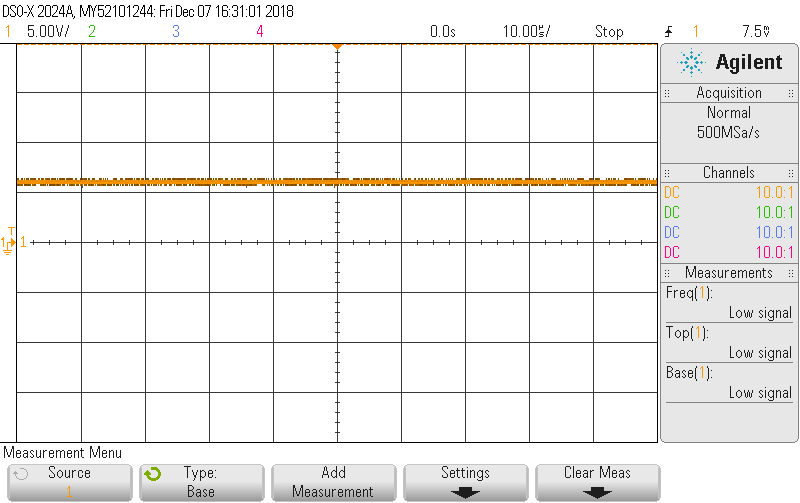
\includegraphics[width=1\textwidth]{billeder/shunt_pos_png.png}
	\caption{Her ses outputtet fra den positive shunt regulator}
	\label{fig:positiv_shunt}
\end{figure}
\subsection{Beregninger}
Indgangsspændingen fra batterierne er $V_{in} = \pm \SI{8.4}{\volt}$. 
For at overskueligegøre beregningerne, anvendes kun den positive spænding, hvoraf komponentværdierne antager samme værdi for den negative spænding, dog bliver zenerdioden forspændt i modsat retning.
Udgangsspændingen ønskes at $V_{out} = 7 \si{\volt}$. 
Indgangsstrømmen vælges til $I_{in} = 20\si{\milli\ampere}$, og bruges til at bestemme udgangsstrømmen.
Zenerdiodens strøm og modstand findes i databladet $I_Z = 5 \si{\milli\ampere}$ $r_z = 15 \si{\ohm}$. \cite[Side. 1 Kolonne 12]{ZenerDiode}

For at der skal ligge en konstant spænding på $7 \si{\volt}$ udregnes først breakdown spændingen over dioden ved at bruge formel \ref{eq:BreakdownVolt} \cite[Side. 146]{Sedra19uu} formlen for spændingen over dioden er den samme som udgangsspændingen på loaden. 
\begin{align}
	V_o & = V_{Z0} + r_z I_z \label{eq:BreakdownVolt} \\
	V_{Z0} & = \SI{6.925}{\volt}
	\end{align}
Værdien $V_{Z0}$ er diodens breakdown spænding.
Breakdown er det punkt hvori spændingsfaldet over dioden er konstant og bliver anvendt til at få en konstant udgangsspænding.
For at beregne modstanden anvendes ligning \ref{eq:RegulatorModstand} \cite[Side. 149]{Sedra19uu}.
\begin{align}
	R_1 & = \frac{V_{in}-V_{Z0}-r_z I_z}{I_z+I_{out}} = 70\si{\ohm} \label{eq:RegulatorModstand}
\end{align}
Modstanden udregnes til $70 \si{\ohm}$, hvoraf den tilnærmede værdi bliver $R_1 = 68 \si{\ohm}$.
Til dette anvendes ligning \ref{eq:UdgangShunt} \cite[Side. 149]{Sedra19uu}.
\begin{align}
	V_{out} & = V_{Z0} \cdot \left( \frac{R_1}{R_1+r_z} \right) + V_{in} \cdot \left( \frac{r_z}{R_1+r_z} \right) - I_{out} \cdot \left( \frac{r_z \cdot R_1}{r_z+R_1} \right) \label{eq:UdgangShunt}
\end{align}
Udgangsspændningen bliver da $V_{out} = \SI{7.04}{\volt}$.

Ovenstående beregninger er udført for en BZX79C6V8 diode. 
Da der blev lavet en endelig komponentliste blev der ved et uheld valgt en BZX79C6V2 diode i stedet for. 
Forskellen her er at den nye diode maksimalt kan holde en konstant spænding på $\SI{6.6}{\volt}$ i udgangsspænding og diode modstanden er $r_z = 10 \si{\ohm}$ \cite[Side. 1 Kolonne 11]{ZenerDiode}.
Ved tilsvarende udregninger findes det frem til at udgangsspændingen er $\SI{6.66}{\volt}$ ved en modstand på $68 \si{\ohm}$.
